\vspace{10pt}

{\centering\subsection*{何锦玉:游柃蜜小镇}}

\addcontentsline{toc}{subsection}{何锦玉:游柃蜜小镇}

\renewcommand{\leftmark}{何锦玉:游柃蜜小镇}

\begin{figure}[htbp]

\centering

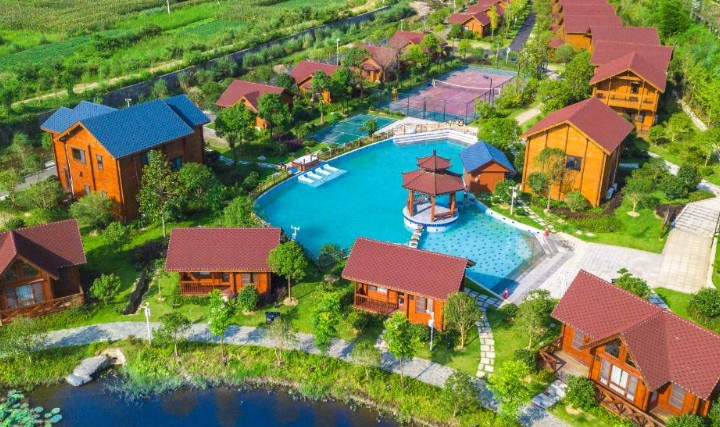
\includegraphics[width = .5\textwidth]{./ch/30.jpg}

\end{figure}




蔚蓝的天空下是那风光无限,多姿多彩的崇阳柃蜜小镇景区,那里有上千层阶梯,直达云霄,又惊险又有名的玻璃桥,和我来看看吧!


进入大门,高高的山岭浮现在眼前,可以看见一个由藤萝组成的爱心门,那边是山路门口,没有缆车,只能徒步攀登,也许只是开发者给游客的考验,山路沿着石壁做成的石壁上长满了草和青苔,不留一丝空隙。


山顶上就是又长又干净的玻璃桥,玻璃桥之所以一干二净,是因为要穿上鞋套,我穿上绿色的鞋套,大踏步的向前走,可一旁的大人却吓的瑟瑟发抖。


玻璃桥过了,又要走一段山路,到了既惊险又刺激的彩虹滑道了,看着前面的孩子大声尖叫,我不由自主的去排队,我按照工作人员的指令躺在已经准备好的“大游泳圈”里,工作人员一推我就从20米长的彩虹滑道上滑下来……


我们再一次走山路,不过这次是下山。


我跑到山脚下,看见了指示牌上的字,动物园,我意外的走到一个笼子前,我惊讶了,我不敢相信我的眼睛看到了一只北极狐,我揉了揉眼睛,又看了看栅栏外的牌子,还真是北极狐,我想他是怎么适应南方的?难道他是动物园里最后一只北极狐?果然我在动物园里走了一圈,还真没见到那一身雪白,尾巴像鸡毛掸子一样的北极狐。


不知不觉中就到了吃午餐的时间了,我们按指示牌上的图片和文字找到的餐厅,吃完饭后都依依不舍的离开了柃蜜小镇。


柃蜜小镇这时虽然没建设完毕,但有哪一个建设完的景点比得过这时柃蜜小镇的丰富多彩,希望你有机会去细细体会。

\vspace{10pt}

作者:四(1)班  何锦玉



指导老师:周瑞




投稿:2021年4月30日



发表:2021年5月6日













\vspace{10pt}

\hline



